\documentclass[10pt]{article}
\usepackage[polish]{babel}
\usepackage[utf8]{inputenc}
\usepackage[T1]{fontenc}
\usepackage{graphicx}
\usepackage[export]{adjustbox}
\graphicspath{ {./images/} }

\title{Akademia \\
 Pomorska \\
 w Stupsku }

\author{}
\date{}


\begin{document}
\maketitle
\begin{center}

\includegraphics[max width=\textwidth]{2024_11_21_3ef8bd11d8ae747125ecg-1(1)}
\end{center}

\begin{center}

\includegraphics[max width=\textwidth]{2024_11_21_3ef8bd11d8ae747125ecg-1(2)}
\end{center}

\section*{LIGA MATEMATYCZNA \\
 im. Zdzisława Matuskiego \\
 FINAŁ 18 maja 2021 \\
 SZKOŁA PODSTAWOWA \\
 klasy IV - VI}
\section*{ZADANIE 1.}
Bartek miał osiem karteczek z cyframi 1, 1, 2, 2, 3, 3, 4 i 4. Próbował ułożyć z nich liczbę parzystą podzielną przez 9. W końcu usunął jedną karteczkę. Z siedmiu pozostałych ułożył liczbę parzystą podzielną przez 9. Wyznacz największą liczbę, którą mógł utworzyć Bartek. Odpowiedź uzasadnij.

\section*{ZADANIE 2.}
W biegu na 100 metrów startuje 625 zawodników. Bieżnia stadionu ma 5 torów i tylko zwycięzca każdego biegu przechodzi do kolejnej rundy, a wszyscy pozostali odpadają z dalszej rywalizacji. Oblicz najmniejszą liczbę biegów konieczną do wyłonienia zwycięzcy zawodów.

\section*{ZADANIE 3.}
Znajdź wszystkie liczby trzycyfrowe, których iloczyn cyfr jest równy 6.

\section*{ZADANIE 4.}
Ania ma 183 zł, a Bartek 75 zł. Ile pieniędzy Ania powinna dać Bartkowi, aby zostało jej dwa razy więcej niż miałby wtedy chłopiec?

\section*{ZADANIE 5.}
Pięć koleżanek z grupy kolonijnej ułożyło kwadrat ze swoich ręczników tak, jak na rysunku. Ręczniki Ani i Basi mają kształt kwadratów, każdy o obwodzie 720 cm. Ręczniki Celiny, Darii i Eli są prostokątami o jednakowych wymiarach. Oblicz obwody prostokątnych ręczników i dużego kwadratu utworzonego ze wszystkich ręczników.\\
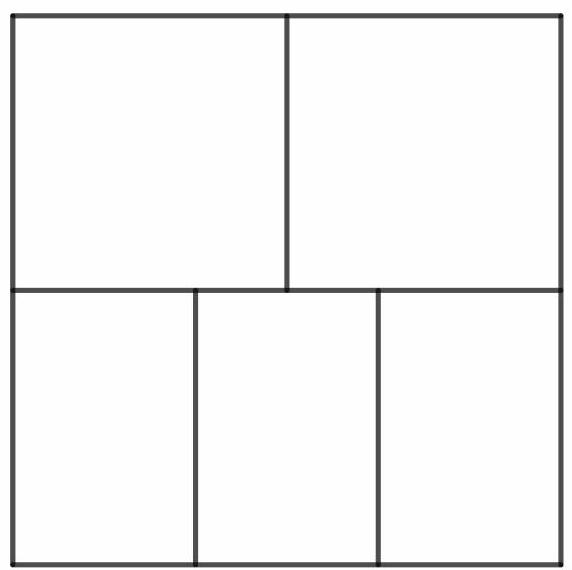
\includegraphics[max width=\textwidth, center]{2024_11_21_3ef8bd11d8ae747125ecg-1}


\end{document}